\documentclass{book}

%%%%%%%%%%%%%%%%%%%% Packages %%%%%%%%%%%%%%%%%%%%

\usepackage[utf8]{inputenc}
\usepackage[T1]{fontenc}
\usepackage[french]{babel}
\usepackage{graphicx}
\usepackage{geometry}
\usepackage{enumitem}
\usepackage{xcolor}
\usepackage{pdfpages}
\usepackage{tikz}
\usepackage{stmaryrd}
\usepackage{amsmath}
\usepackage{lmodern}
\usepackage{amssymb}
\usepackage{mathrsfs}
\usepackage{colortbl}
\usepackage{mathabx}

%%%% Pour toc %%%%
\addtocounter{tocdepth}{3}
\setcounter{secnumdepth}{3}
\addcontentsline{toc}{section}{Introduction}
\addcontentsline{toc}{section}{Remerciements}
\addcontentsline{toc}{section}{Citations}
\renewcommand{\thesection}{\arabic{section}}

%%%%%%%%%%%%%%%%%%%% Page de Garde %%%%%%%%%%%%%%%%%%%%
\title{%
\begin{minipage}\linewidth
        \centering\bfseries\sffamily
        \Large{INSERM U970 PARCC (Paris Centre Cardiovascualaire)}
        \vskip3pt 
        E04 : Integrative Epidemiology of Cardiovascular Deseases
    \end{minipage}}
\author{\textbf{Odélia Guedj} odelia-g@hotmail.fr \\ M1 Mathématiques en Interaction \\ Université Evry Val d'Essonne}
\date{01/04/2019 - 31/08/2019}

\makeatletter
\let\mytitle\@title
\let\myauthor\@author
\let\mydate\@date
\makeatother

\begin{document}
\begin{titlepage}

\enlargethispage{10 cm}


\includegraphics[scale = .4]{logo_inserm.jpg}\hfill

\includegraphics[scale = .2]{logo_parcc.jpg}\hfill

\includegraphics[scale = .4]{logo_ueve_saclay.png}
\\ \\ \\ \\ \\ \\ \\ \\ \\ \\

\bigskip
\begin{center}
\Huge{\textbf{Rapport de stage M1}}\\
\bigskip
\mytitle \\
\bigskip
\normalsize{\textbf{\mydate}}\\
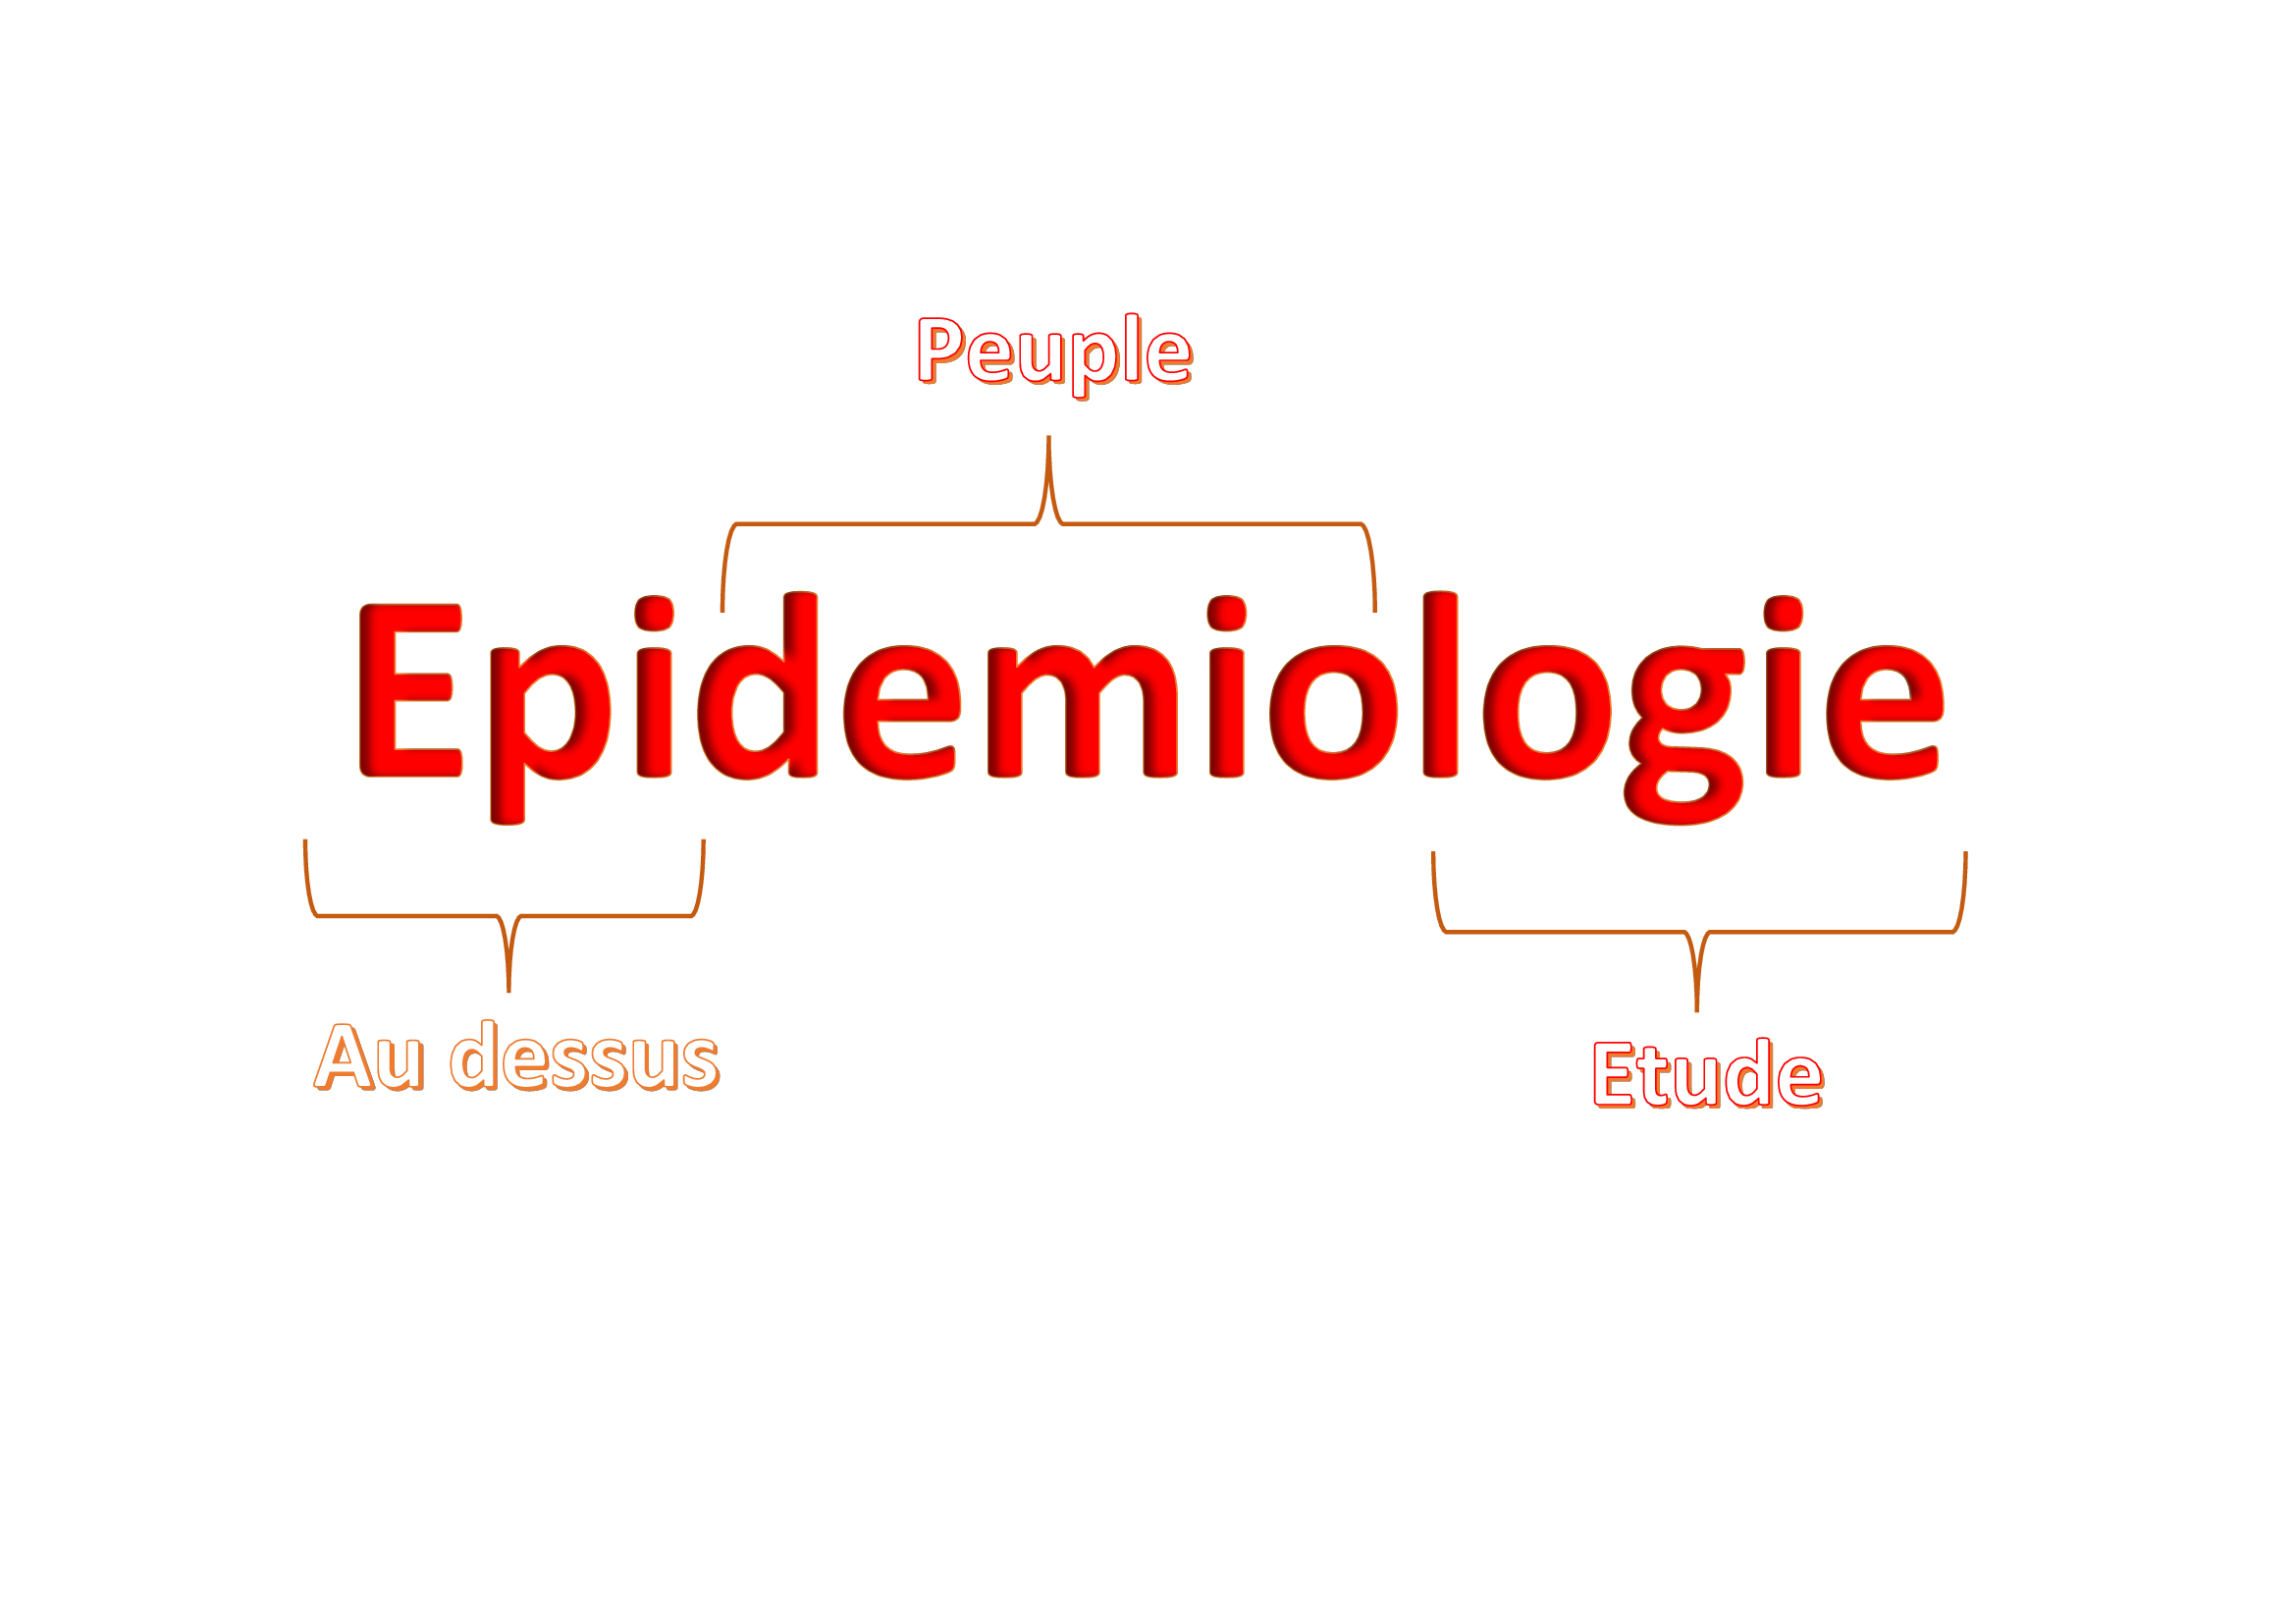
\includegraphics[scale= .15]{Epidemiologie_logo_r.png}

\end{center}
\begin{center}
\begin{flushleft}
\myauthor 
\end{flushleft}

\begin{flushright}
\textbf{Dr Jean Philippe Empana} \\
Research Director, MD, PhD \\
INSERM U970 PARCC
\end{flushright}
\end{center}

\end{titlepage}
 
%%%%%%%%%%%%%%%%%% frontmatter %%%%%%%%%%%%%%%%%%%
\frontmatter

\tableofcontents

\newpage
\begin{center}
\section*{Remerciements}
\end{center}

\newpage
\begin{center}
\section*{Citations}
\end{center}
\newpage



%%%%%%%%%%%%%%%%%%%% main matter %%%%%%%%%%%%%%%%%%%%%%%%%%%%%%%%
\mainmatter


\newpage
\begin{center}
\section*{Introduction}
\end{center}


\newpage
\section{Contexte}
\subsection{L'Inserm U970 Equipe 4}
\subsection{L'Etude Parisienne Prospective 3 (EPP3)}
\noindent
EPP3 est une étude prospective de cohorte en population générale comptant n = 10157 sujets.\\
Ces dernier ont été recrutés dans des centres IPC (centres d'examens de santé conventionnés par l'assurance maladie) entre Juin 2008 et Décembre 2011.\\
Pour entrer dans l'étude, les sujets doivent avoir entre 50 et 75 ans.\\
\\
Les donnés sont récoltées via des questionnaires envoyés tous les deux ans qui, à l'exception du questionnaire d'inclusion sont élaborés à l'INSERM U970 équipe 4. \\
Le questionnaire d'inclusion provient de l'IPC. Il contient une partie socio-admnistrative, des question sur l'environnement professionnel des sujets ainsi que sur leurs habitudes de vie (alimentation, tabac, alcool). 
Une autre partie du questionnaire traite des antécédents médicaux des sujets, tant familiaux que personnels, de leur état de santé actuel et de leurs prescriptions médicamenteuses.
La dernière partie traite du bien-être des sujets: on y trouve des questions sur leur stress perçu, leur équilibre mental ainsi que leur nutrition.\\
\\
Le but de l'étude est la recherche de facteurs de risque pour les maladies cardiovasculaires.\\ 
Dans chacun des questionnaires il est demandé aux sujets de déclarer leurs hospitalisations en détaillant le motif d'hospitalisation, le nom de l'hôpital, du service où ils ont été traités ...
Chaque hospitalisation déclarée est appelée évènement.\\
\\
Pour s'assurer de la validité des déclarations des sujets, un protocole de validation d'événement a été mis en place : régulièrement un certain nombre d'événements sont extraits de la base. Pour chaque évènement, on contacte l'hôpital pour qu'il transmette au responsable de l'étude les comptes-rendus hospitaliers (CRH) de l'évènement en question. Ensuite les CRH sont lus par un médecin qui valide, invalide ou corrige le diagnostique déclaré par le sujet.\\
\\
L'étude EPP3 est une étude longue, il est prévu que le suivi dure 20 ans (10 questionnaires à raison d'un tous les deux ans).\\
Elle a déjà donné lieu à la publication de plus d'une vingtaine d'articles dans des revues prestigieuses comme le JACC (Journal of the American College of Cardiology) ou le JAMA (Journal of the American Medical Association).
\subsection{Sujet de stage : Définition et limites}

\newpage
\section{Bref aperçu de l'épidémiologie}
\subsection{Histoire et définition}
\subsection{Vocabulaire indispensable (analogie avec le vocabulaire "orienté mathématiques")}
\subsection{Principaux biais et indicateurs de l'épidémiologie}

\newpage
\section{Description et explication des données}
\subsection{Variable d'expostion : activpro}
Dans le questionnaire d'inclusion, 3 questions traitent de l'activité professionnelle des sujets (Question 1,2,3 du questionnaire IPC en annexe). Ces 3 questions ont été codées en 4 variables catégorielles :

\begin{itemize}[label=\textbullet, font=\small \color{red} ]

\item Adm12 : Êtes-vous
\begin{itemize}[label=\textbullet, font=\small \color{blue} ]
\item 6NNNNN  contrat emploi-solidarité, intérim, CDD
\item N5NNNN  chômeur depuis + de 6 mois
\item NN4NNN  chômeur depuis - de 6 mois
\item NNN3NN  à la recherche d'un emploi
\item NNNN2N  jeune en cours de formation
\item NNNNN1  étudiant
\end{itemize}
\bigskip
\item Adm12a : Êtes-vous
\begin{itemize}[label=\textbullet, font=\small \color{blue} ]
\item JXXX  en formation professionnelle
\item X9XX  au foyer
\item XX8X  retraité(e)
\item XXX7  pré-retraité(e)
\end{itemize}
\bigskip
\item Adm11 : Depuis quand n'exercez-vous plus d'activité professionnelle ?
\begin{itemize}[label=\textbullet, font=\small \color{blue} ]
\item 0	en activité
\item 1	moins d'un an
\item 2	1 an
\item 3	2 ans
\item 4	3 ans ou +
\item 5	jamais travaillé
\end{itemize}
\bigskip
\item Adm10 : Si vous travaillez quelle est votre profession ? \\
La réponse à cette question est du texte libre. Après la récupération des questionnaires par l'IPC, un code à deux chiffres est attribué à chaque grand groupe de profession. 
\end{itemize}

\noindent
L'encodage de la variable Adm10 introduit une première source potentielle d'erreur du fait de la difficulté d'interpréter du texte libre d'une part et des possibles erreurs de "classification humaine" d'autre part. J'ai été confronté à ces dernières lors du codage de ma variable d'exposition. Nous y reviendrons au paragraphe suivant. Il faut également noter qu'un des sujets a un code travail de 88 et que ce code ne correspond à aucune des professions de la liste IPC (en annexe).

\noindent
Une autre difficulté est due à la possibilité qu'ont les sujet de cocher plusieurs réponses par question. Il en résulte un grand nombre de classes dans chaque variable ce qui a compliqué le codage de la variable activpro.

\subsubsection{Codage manuel}
\noindent
L'objectif du projet étant d'étudier l'impact de l'activité professionnelle sur la santé perçue des sujets, il faut tout d'abord résumer l'information contenue dans les 3 variables citées précédemment en une seule variable.

\noindent
J'ai donc créer une variable catégorielle nommée activproManuel qui comporte 5 classes:
\begin{itemize}[label=\textbullet, font=\small \color{black} ]
\item R pour retraités
\item T pour travailleur
\item C pour chômeur
\item I pour inactif
\item NSP pour ne sait pas (cas "inclassables")
\end{itemize}

\noindent
Pour cela j'ai fait le choix de me baser de manière successive sur les variables Adm12a puis Adm11 puis Adm12 puis Adm10. La raison en est simple : c'est la variables Adm12a qui propose la réponse "Retraités", or c'est la catégorie qu'il m'intéresse le plus d'étudier. Ensuite la variable Adm11 nous indique si le sujet travaille encore OU depuis combien de temps il a cessé de travailler. La variable Adm12 discrimine les chômeurs. Enfin, la variable Adm10 est utile pour vérifier la cohérence des différentes réponse des sujets ou bien de trancher dans des cas où les autres variables ne fournissaient pas d'informations suffisantes.\\
Par exemple, il y a 57 individus pour lesquels les variables Adm12 et Adm12a ne sont pas renseignées et qui déclarent ne plus travailler depuis moins d'un an ou plus (c'est à dire qu'ils ont cochés les cases 1,2,3,4 ou 5 du questionnaire). Il est possible que ces sujets soient au chômage, à la retraite ou qu'ils n'aient jamais travaillé.\\
\newline
Voici le tableau récapitulant comment ont été classés ces sujets en fonction de leur code travail:\\
\begin{center}
\begin{tabular}{l|l}
 & Codes \\
 \hline
Retraités & 71 72 73 74 75 76 77 78\\
Chômeurs & 91 92 93 94 95 96\\
Inactifs & 81 82 84 85 86\\
Ne sait pas & 88\\
Travailleurs & Le reste
\end{tabular}
\end{center}


\noindent
\textbf{Règle de décision} : 
Les sujets indiquant qu'ils sont à la retraite et qu'ils travaillent sont classés en tant que travailleurs et ce, même si leur code travail (c'est à dire la variable Adm10) est de type "Ancien X" (codes 71 à 78 de la liste IPC) car il est possible de percevoir une pension de retraite et de continuer à travailler (par exemple en tant qu'expert). Or ce qui est intéressant pour l'étude est la santé perçue des sujets ne travaillant plus du tout. Il vaut donc mieux classer ceux qui complètent leur retraite avec un emplois en tant que travailleurs qu'en tant que retraités.

\noindent
Ainsi, sont étiquetés inactifs les sujets n'aillant jamais travaillé, ou déclarant être au foyer ou ayant un code travail parmi les deux suivants : 85/86. Ces codes correspondent à des individus inactifs non retraités respectivement de moins de 60 ans et de plus de 60 ans.

\noindent
Si les variables Adm12 OU Adm10 indiquent que le sujet est chômeur (en incluant la simple recherche d'emplois), il est classé en chômeur.En effet, on peut raisonnablement faire l'hypothèse que la précarité induite par la recherche d'un emplois occasionnera une plus mauvaise santé perçue.

\noindent
On classe retraités tous les sujets n'ayant aucun indicateur de chômage ou d'activité professionnelle et n'étant pas inactifs.

\noindent
Enfin, le reste est classé comme travailleurs.

\noindent
Malgré toutes les étapes de la classification et la minutie des vérifications, il  existe un certain nombre de cas "impossibles" à classer car les informations d'un sujet pour les différentes variables sont contradictoires Ces sujets sont étiquetés NSP.\\

\noindent
Finalement on obtient la répartition suivante : \\
\bigskip
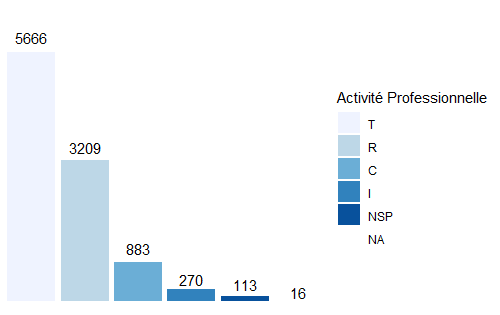
\includegraphics[scale=1]{activpro_barplot_manuel.png}

Pour vérifier la cohérence des classes obtenues on peut tracer les distributions de l'âge dans chaque classe.

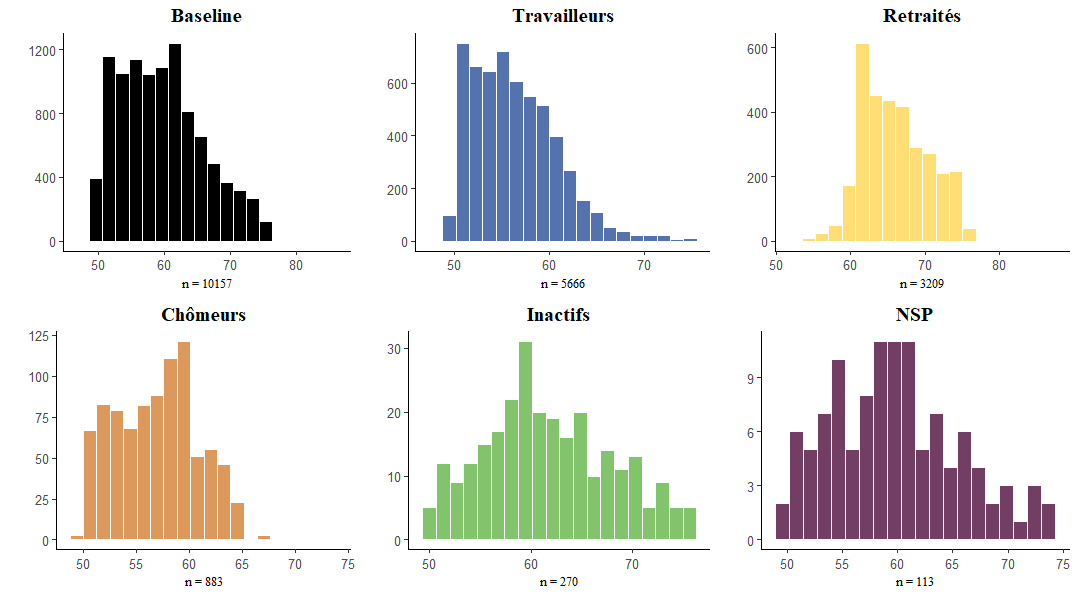
\includegraphics[scale=1.3]{plot_grid_hist_age_activproBis.png}\\

On remarque que 1116 sujets classés Travailleurs ont moins de 60 ans (on peut raisonnablement supposer que l'âge de la retraire est 60 ans car les sujets de la cohorte ont, à l'inclusion, un âge compris entre 50 et 75 ans).
De même, 134 sujets sont classés en tant que Retraités et ont moins de 60 ans.

Ceci peut s'expliquer soit par une erreur de classification: ayant effectué cette dernière à la main il y a un risque non négligeable que je n'ai pas appliqué exactement le même critère de jugement pour chacun des cas. Il peut aussi ne pas s'agir d'une erreur dans ce cas les données sont ainsi et on veillera simplement à garder cela à l'esprit lorsque nous interpréterons les résultats des tests statistiques ultérieurs.


\subsubsection{ACM et CAH}
\noindent
Pour vérifier la cohérence des résultats présentés au paragraphe précédent, j'ai effectué une Classification Ascendante Hiérarchique sur une base de données constituée des quatre variables utilisées pour la classification "manuelle" : Adm12a, Adm11, Adm12 et Adm10. \\
J'ai également veillé à supprimer les individus (n = 29) ayant une valeur manquante pour l'une de ces quatre variables. 
Les résultats de l'ACM sont rassurants, dans le sens où l'emplacement des quatre variables qui nous intéressent dans le plan factoriel correspond à l'intuition qu'on en avait à savoir : 
\begin{itemize}
\item Les variables Adm12a et Adm11 apportent globalement la même information, cohérent puisque Adm12a et Adm11 discriminent les retraités et les travailleurs.
\item Adm12 et Adm10 sont sur le même plan horizontal : elles discriminent les chômeurs (avec les codes travail 91 à 96).
\item Adm12a, Adm10 sont dans le même plan vertical : elles discriminent les inactifs.
\end{itemize}
On s'attend donc à ce que la CAH effectuée sur les résultats de l'ACM produise une classification proche de celle effectuée à la main.\\
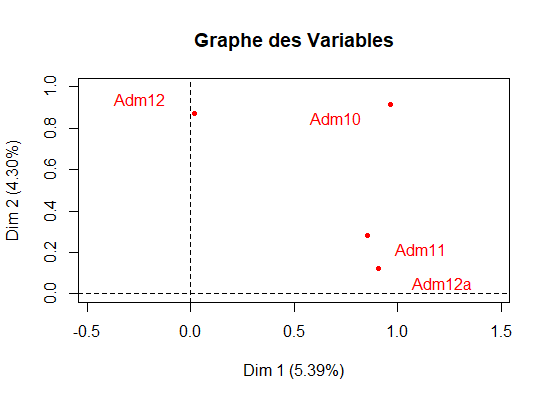
\includegraphics[scale = 1]{ACM_var.png}

\noindent
\textbf{NB:}Les faibles pourcentages d'inertie sont tout à fait normaux dans le cadre d'une ACM. En effet, comme l'explique Jérôme Pagès dans son livre "Analyse factorielle multiple avec R", si les variables étaient toutes identiques dans le cas d'une ACP la première dimension aurait 100\% d'inertie alors que dans une ACM la première dimension aurait au maximum $100\over{(nb_modalités - 1)}$ \% d'inertie.\\

\noindent
Sur le graphe suivant on affiche les individus ainsi que les 15 modalités ayant la plus grande contribution. Ces 15 modalités sont affichées selon un gradient de couleur en fonction de leur cos2. \\
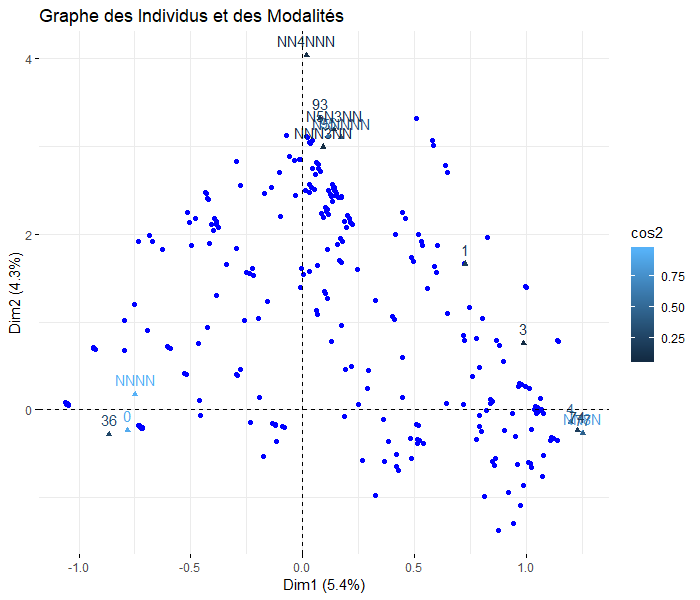
\includegraphics[scale = 1]{ACM_var_ind.png}

On voit de façon assez claire trois groupes distincts : le premier en bas à droite est certainement celui des sujets retraités, on y retrouve les modalités 1,3,4 de Adm11 (ne travaille plus depuis resp, moin de 1 an, deux ans, trois ans et plus), 74 de Adm 10 (Ancien cadre), NN8N de Adm12a (Retraité).\\
Le groupe en haut correspond sans doute aux chômeurs puisque les modalités NNN3NN, NN4NNN et N5N3NN de Adm12 (resp. A la recherche d'un emploi , Chômeur depuis moins de 6 mois et A la recherche d'un empois + Chômeur depuis 6 mois) et 93 de Adm10 (cadres et professions intellectuelles chômeurs).\\
Enfin le dernier groupe est celui en bas à gauche, il représente surement les travailleurs puisque la modalité 0 de Adm11 s'y trouve (Travaille) ainsi que 36 de Adm10 (Cadres) et NNNN de Adm12a. La présence de cette dernière modalité fait sens puisqu'elle représente les individus n'ayant rien coché dans la variable Adm12a doit les choix étaient pré-retraités, retraités, personne au foyer, en formation professionnelle. Or si ces sujets travaillent, aucune de ces catégories ne les concerne.\\
Il reste deux choses qu'il me semble pertinent de relever: l'ACM semble particulièrement discriminer les cadres, on les retrouve dans les chômeurs, les retraités et les travailleurs. Ceci s'explique par le fait que les modalités 36, 74 et 93 (resp Cadres d'entreprises, Anciens cadres et Cadres et professions intellectuelles chômeurs) représentent à elles seules 3848 sujets (sur 10157 sujets dans la base globale et 10128 dans la base ayant permis l'ACM).\\
La deuxième chose à noté est l'absence d'un quatrième groupe qui aurait représenté les inactifs. Une explication possible est la faible proportion de ces sujets dans la base. En effet lors de la classification manuelle on n'avait étiqueté "que" 270 sujets comme inactifs. \\

\noindent
La question que je me suis ensuite posée est celle de l'allure qu'aurait ma classification si elle était effectuée par un algorithme. De plus, il serait intéressant d'analyser la classification des individus que je n'ai pas su classer.
Pour cela j'ai effectué une Classification Ascendante Hiérarchique avec le package FactomineR de R en choisissant la distance du chi-deux et le critère d'agrégation de Ward.\\

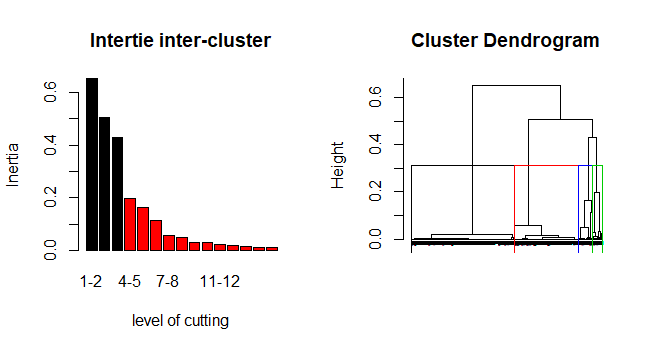
\includegraphics[scale = 1]{dendro_inertie_cah.png}\\
Le graphe d'inertie semble indiquer que le nombre idéal de clusters est 4. On peut voir sur le dendrogramme que c'est effectivement le nombre de clusters retenu ce qui est bon signe puisque l'idée était de repartir tous les sujets en 4 groupes : travailleurs, retraités, chômeurs et inactifs.
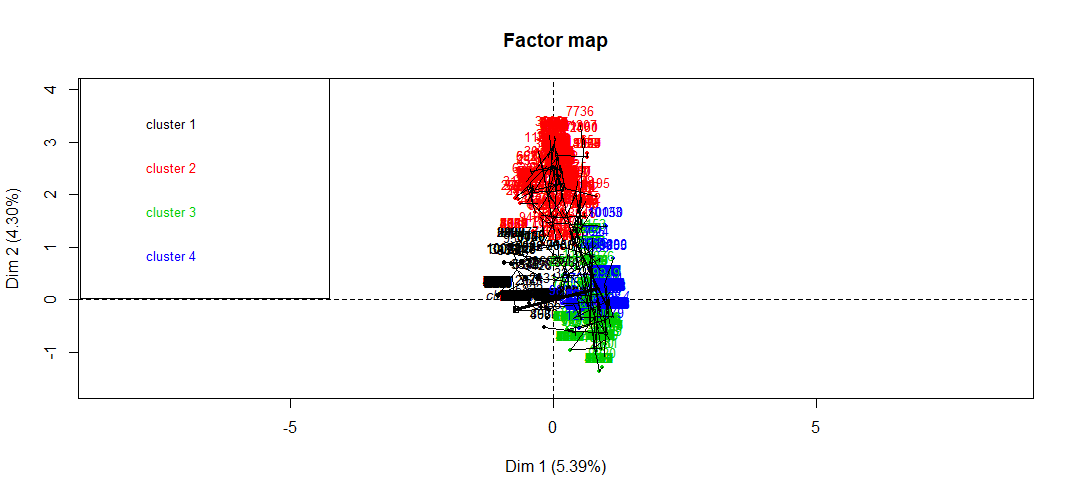
\includegraphics[scale = .5]{cah_ind_cluster.png}

Pour pouvoir interpréter les cluster obtenus par la CAH il est indispensable de comprendre quelles sont les modalités qui contribuent le plus à chaque cluster.\\
Pour cela on cherche à déterminer si la forte présence d'une modalité dans un Cluster est due au hasard. Dans le cas contraire cela signifie que la modalité est représentative du Cluster.\\\\

On effectue le test suivant pour chaque modalité dans chaque cluster:
\noindent 
$H_0$ : La proportion de la modalité m dans le cluster c est due au hasard
\noindent
$H_1$ : La proportion de la modalité m est anormalement élevée/basse dans le cluster c.\\

\noindent
Ainsi sous $H_0$ on a : 
${{n_{mc}} \over {n_c}} = {{n_m} \over {n}} $ où :\\
$n_{mc}$ est le nombre de sujet du cluster c présentant la modalité m,\\
$n_c$ est le nombre de sujets dans le cluster c,\\
$n_m$ est le nombre de sujets présentant la modalité m,\\
$n$ est le nombre total d'individus.\\
	
\noindent
Sous $H_0$ : $n_{mc}  = {n_m . n_c \over {n}} $\\
Or le rapport ${n_m . n_c \over {n}} $ suit une loi hypergéométrique.\\
Soit $N_{mc}$ la variable aléatoire représentant l nombre d'individus de la modalité m dans le Cluster c.
\begin{equation}
 N_{mc} \underset{H0}{\sim} \mathcal{H}(n, n_c, {{n_m}\over {m}})
\end{equation}

\noindent
La fonction catdes() du package factoMineR nous résume les résultats de ce test pour chaque modalité dans chacun des clusters en classant les modalité dans l'ordre décroissant de leur contribution au cluster.
Seuls les test significatifs sont affichés.\\

\noindent
Dans les résultats affichés juste aprés, la première colonne correspond au nom de la modalité, la deuxième calcule le rapport $n_{mc} \over n_m$, la troisième le rapport $n_m \over n_c$, la quatrième le rapport $n_{mc} \over n$.\\
La cinquième colonne est le calcul de la p-valeur :\\
\begin{equation}
\mathbb{P}_{H0}(N_{mc} \geq n_{mc, obs}) =  \mathbb{P}_{\mathcal{H}(n, n_c, {n_m \over n})}(N_{mc} \geq n_{mc, obs})
\end{equation} 
Enfin, la dernière colonne est la valeur de la statistique de test calculée. Lorsqu'elle est positive la modalité à laquelle elle est associée est sur représentée dans le Cluster et lorsqu'elle est négative le modalité en question est sous représentée dans le Cluster.\\*

\noindent
Par souci de lisibilité nous n'afficheront que les modalités surreprésentée dans chaque cluster:

\setlength\arrayrulewidth{2pt}
\arrayrulecolor{black}
\begin{tabular}{|c||ccccc|}
\hline
  \textbf{\textcolor{black}{Cluster 1}}       &    Cla/Mod  &   Mod/Cla   &   Global   &    p.value  &   v.test  \\
\hline
\hline 
            
Adm12a=NNNN  & 87.25 &99.91 &61.73  &0 &       Inf\\
Adm11=0      & 92.41 &99.29 &57.92  &0 &       Inf\\
Adm10=36     & 99.88 &46.21 &24.94  &0 &      Inf\\
Adm10=54     & 99.62 &14.41 & 7.80 &3.80e-217  &31.45\\
Adm12=NNNNNN & 57.94 &97.60 &90.82 &7.30e-155 & 26.51\\
Adm10=51     & 100 & 9.03 & 4.87 &1.12e-137  &24.98\\
Adm10=32     & 99.78 & 8.19 & 4.42 &3.78e-122  &23.50\\
Adm10=61     & 100 & 6.01 & 3.24 & 9.09e-91 & 20.20\\
Adm10=56     & 100 & 3.86 & 2.08 & 3.58e-58 & 16.08\\
Adm10=66     & 100 & 3.59 & 1.94 & 4.94e-54 & 15.48\\
Adm10=47     & 99.28 & 2.53 & 1.37 & 2.75e-36 & 12.58\\
Adm10=48    & 100 & 2.20 & 1.18 & 3.43e-33 & 12.00\\
Adm10=55    & 100& 1.41 & 0.76 & 1.70e-21 &  9.52\\
Adm12=6NNNNN & 80.52 & 2.27 & 1.52 & 4.19e-12  & 6.93\\
Adm10=41    & 100 & 0.77 & 0.41 & 4.99e-12 &  6.91\\
Adm10=46    & 100 &0.51 & 0.28 & 2.97e-08 &  5.54\\
\hline
\end{tabular}

\bigskip
Les modalités de la variable Adm10 sur représentées dans le \textbf{\textcolor{black}{Cluster 1}} correspondent toutes à des codes travail de sujet qui travaillent. La modalité la plus présente dans ce Cluster est Adm12a = NNNN, c'est à dire les sujets n'ayant coché aucune modalité de cette variable. Cela fait sens puisqu'aucune des modalités possibles ne traitaient d'une activité professionnelle. Enfin les modalités de la variable Adm12 représentées dans le Cluster 1 sont NNNNNN c'est à dire ceux n'ayant rien coché et 6NNNNN : en contrat emplois-solidarité / intérim / CDD.


\bigskip
\setlength\arrayrulewidth{2pt}
\arrayrulecolor{red}
\begin{tabular}{|c||ccccc|}
\hline
 \textbf{\textcolor{red}{Cluster 2}}            &    Cla/Mod  &   Mod/Cla   &   Global   &    p.value  &   v.test  \\
\hline
\hline 
   
Adm12=N5NNNN  &99.74 &45.49 & 3.79 & 0   		&     Inf\\
Adm10=95      &98.52 &71.14 & 6.00 & 0  		&      Inf\\
Adm10=93      &100   &17.93 & 1.49 &1.42e-169 	&27.76\\
Adm12=N5N3NN  &100   &17.81 & 1.48 &2.05e-168  &27.66\\
Adm12a=NNNN   &12.59 &93.47 &61.73 &1.89e-108  &22.12\\
Adm11=1       &37.58 &28.38 & 6.28 &1.39e-103  &21.61\\
Adm12=NNN3NN  &90.65 &11.52 & 1.06 & 1.38e-94  &20.63\\
Adm12=NN4NNN  & 100  &7.13 & 0.59 & 2.13e-66  &17.21\\
Adm10=96      & 82.95 & 8.6698337 & 0.86887836 & 7.223367e-65  &17.007518\\
Adm12=NN43NN& 100 & 4.9881235 & 0.41469194 & 1.646295e-46  &14.319786\\
Adm12a=NNN7   &55.56 & 5.9382423 & 0.88862559 & 6.429777e-31  &11.561864\\
Adm11=2       &26.68 &13.1828979 & 4.10742496 & 3.196727e-30  &11.423349\\
Adm11=3       &24.17 &14.6080760 & 5.02567141  &5.036790e-29  &11.181263\\
Adm10=94      &100 & 1.3064133 & 0.10860979  &1.234652e-12  & 7.101438\\
Adm12=65NNNN  &78.57 & 1.3064133 & 0.13823065  &3.632761e-10  & 6.269042\\
Adm12=6NN3NN  &70 & 0.8313539 & 0.09873618  &2.657340e-06  & 4.695670\\
Adm11=4       &10.34&32.5415677 &26.15521327  &1.612450e-05  & 4.312738\\
Adm12=65N3NN  &100 & 0.4750594 & 0.03949447  &4.745827e-05  & 4.067804\\
Adm12=6NNNNN & 17.53 & 3.2066508 & 1.52053712  &2.141441e-04  & 3.701718\\
Adm12=6N43NN &100 & 0.3562945 & 0.02962085  &5.727234e-04  & 3.444213\\
Adm12a=JNNN  & 66.67 & 0.2375297  &0.02962085  &2.013941e-02  & 2.323740\\
\hline
\end{tabular}


\bigskip

Dans le \textbf{\textcolor{red}{Cluster 2}}, les codes travail présents sont 94/93/94 : ils correspondent aux sujets chômeurs. De plus la modalité la pus représentée dans ce cluster est Adm12 = N5NNNN : sujes chômeurs depuis plus de 6 mois. Toutes les autres modalités de Adm12 résentent dans le Clusteur concernent également des chômeurs. Concernant la variable Adm11, les modalités présentes sont 1,2,3,4 c'est à dire les sujets ne travaillant plus depuis au moins moins d'un an. On remarque aussi que certains sujets en formation professionnelle (Adm12a = JNNN) sont inclus dans le Cluster. 

\bigskip

\setlength\arrayrulewidth{2pt}
\arrayrulecolor{green}
\begin{tabular}{|c||ccccc|}
\hline
 \textbf{\textcolor{green}{Cluster 3}}   &    Cla/Mod  &   Mod/Cla   &   Global   &    p.value  &   v.test  \\
 \hline
 \hline
 Adm12a=N9NN &  99.41348974& 81.4903846 & 3.36690363 & 0.000000e+00    &    Inf\\
Adm10=85     & 98.25174825 &67.5480769  &2.82385466 & 0.000000e+00   &     Inf\\
Adm10=86     & 85.00000000 &28.6057692  &1.38230648 &3.761709e-149  &26.010557\\
Adm11=5      & 94.23076923 &11.7788462  &0.51342812  &1.364674e-65  &17.104886\\
Adm11=4      &  8.72027180 &55.5288462& 26.15521327  &2.065844e-38  &12.959875\\
Adm12a=NNN7  & 36.66666667 & 7.9326923 & 0.88862559  &2.674663e-23  & 9.944143\\
Adm12=NNNNNN &  4.46836269 &98.7980769 &90.81753555  &2.729090e-12  & 6.991013\\
Adm12a=N9N7  &100.00000000  &1.6826923 & 0.06911532  &1.878666e-10  & 6.370945\\
Adm12a=N98N  & 66.66666667 & 1.4423077 & 0.08886256  &3.567252e-07  & 5.090710\\
\hline
\end{tabular} 

\bigskip

\noindent
Dans le \textbf{\textcolor{green}{Cluster 3}} la modalité la plus significativement représentée est Adm12a == N9NN : les personnes au foyer. On trouve également des sujet se déclarant en pré retraite (Adm12a = NNN7/N9N7 ou à la retraite(Adm12a = N98N).
Les seules modalités de la variables Adm10 dans ce cluster sont 85/86 ce qui semble indiquer que le cluster correspind à celui des inactifs.
Enfn on remarque que plus de 94 \% des personnes declarant n'avaoir jamais travaillé sont dans e groupe (Adm11 = 5).

\bigskip

\setlength\arrayrulewidth{2pt}
\arrayrulecolor{blue}
\begin{tabular}{|c||ccccc|}
\hline
   \textbf{\textcolor{blue}{Cluster 4}} &Cla/Mod  &   Mod/Cla      &Global      & p.value  &   v.test\\
   \hline
   \hline
Adm12a=NN8N &  99.09462617 &99.50146628 &33.80726698 & 0.000000e+00  &      Inf\\
Adm11=4      & 79.84144960 &62.02346041 &26.15521327 & 0.000000e+00  &      Inf\\
Adm10=77      &98.61687414 &62.72727273 &21.41587678 & 0.000000e+00  &      Inf\\
Adm10=74      &99.57301452 &34.19354839 &11.56200632 & 0.000000e+00  &      Inf\\
Adm12=NNNNNN  &36.98630137 &99.76539589 &90.81753555 &1.996276e-159  &26.903543\\
Adm11=3       &72.88801572 &10.87976540  &5.02567141 & 7.490306e-77  &18.554571\\
Adm11=2       &69.23076923 & 8.44574780  &4.10742496 & 1.427574e-51  &15.108309\\
Adm11=1       &57.70440252 &10.76246334  &6.27962085 & 1.321276e-37  &12.816748\\
Adm10=78     &100.00000000 & 2.05278592  &0.69115324 & 5.014862e-34  &12.160988\\
Adm10=75     &100.00000000 & 0.79178886  &0.26658768  &1.604994e-13 &  7.378154\\
\hline
\end{tabular}

Enfin pour le \textbf{\textcolor{blue}{Cluster 4}} on s'attends à trouver des sujets retraités. En effet, la modalité la plus significativement représentée est Adm12a = NN8N : sujets retraités. Les codes travail intervenant (Adm10 sont 77/74/78/75 : uniquement des codes de la forme "Ancien \textit{profession}".
En outre on ne trouve dans ce cluster aucun individu déclarant travailler (Adm11 = 0 ou Adm12 = 6NNNNN).\\

\noindent
On peut alors conclure que  \textbf{le Cluster 1 correspond aux travailleurs}, \textbf{\textcolor{red}{le Cluster 2 aux chômeurs}}, \textbf{\textcolor{green}{le Cluster 3 aux inactifs}} et \textbf{\textcolor{blue}{le Cluster 4 aux retraités}}.\\
On remarque alors que l'emplacement des Clusters dans le plan factoriel (cf graphe) correspond à l'emplacement des variables dans ce même plan et que nous avons commenté plus haut.

\subsubsection{Comparaisons des deux codages}
\noindent
Étudions las différences entre la classification manuelle et la Classification Ascendante Hiérarchique.\\
Tout d'abord on classe comme NA tous les sujets qui avaient une valeurs manquante pour au moins une des quatre variables ayant servies à la classification (n = 29).\\
On a alors : \\

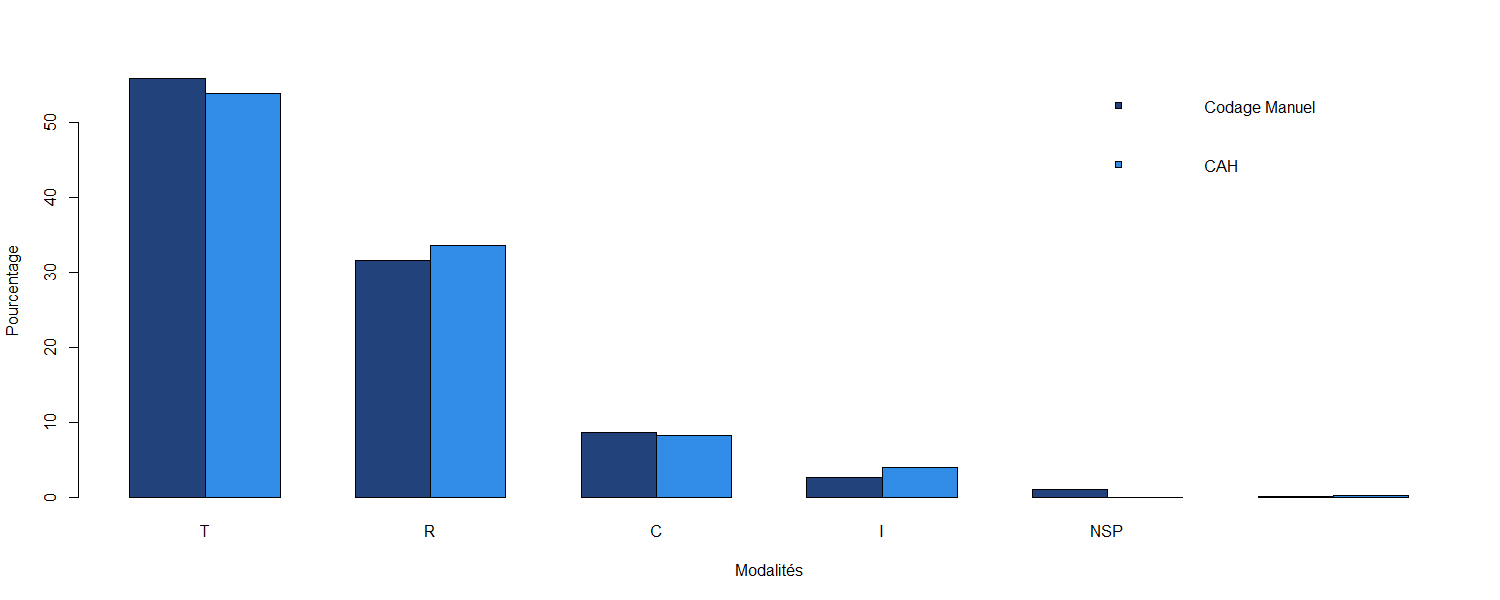
\includegraphics[scale=1]{comp_codages_activpro_pourcentage.png}

\begin{center}
\setlength\arrayrulewidth{.5pt}
\arrayrulecolor{black}
\begin{tabular}{c|cccccc}

	& T & R & C & I & NSP & NA \\
	\hline
activproManuelle & 5666 & 3209 & 883 & 270 & 113 & 16 \\
activproCAH	 & 5460 & 3410 &  842 & 416 & 0 & 29 \\
\hline
\hline
Différence & 206 & -201 &  41 & -146& 113& -13
\end{tabular}
\end{center}

\noindent
Il y a 509 sujets pour lesquels les deux classifications ne correspondent pas. Sur un total de 10157 cela représente 5,01 \% des sujets.\\
On remarque que la classification Ascendante Hiérarchique a tendance à classer plus facilement les sujets en Retraités et en Inactifs et la classification manuelle en Travailleurs. Une raison simple à cette différence est sans doute la volonté d'être le plus restrictifs possible quant à la classification manuelle des retraités.

\noindent
Le nombre de valeurs manquantes n'est pas le même pour les deux classifications pour une raison simple: les 16 NA de la classification manuelle sont des sujets pour lesquels TOUTES les variables nécessaires à la classification (Adm12a, Adm11, Adm12 et Am10) étaient manquantes alors que j'ai dû, pour activproCAH, classer en NA les sujets pour lesquels AU MOINS UNE des 4 variables étaient manquantes afin de pouvoir réaliser l'ACM.

\noindent
Il peut également être intéressant d'étudier la manière dont les sujets classés NSP (n = 113) par la classification manuelle ont été classés par la CAH :\\

\begin{center}
\setlength\arrayrulewidth{.5pt}
\arrayrulecolor{black}
\begin{tabular}{|c|c|c|c||c|}
\hline
R & I & C & T & Total\\
\hline
5 & 77 & 0 & 31 & 113\\
\hline
\end{tabular}
\end{center}

\noindent
Sur quels critères la CAH s'est-elle basée pour classer ces 113 sujets ? 
Pour le comprendre on s'interesse aux trois modalités dans lesquels elle a répartis les NSP (I,R,T) en construisant des Tableaux de Burt et des arbres de décision.\\
Par souci de lisibilité j'ai choisis de n'inclure dans les tableaux de Burt que les modalités contenant un nombre de sujets non nul.\\
Les cases en rouge correspondent simplement aux tableaux de contingences usuels (croisement des variables deux à deux).\\
Le tableaux est évidement "symétrique", j'ai choisi de n'en remplir que la partie inférieure.\\
Concernant les arbres , j'ai reproduit les étapes de classification de la CAH (en fixant l'ordre des 4 variables comme étant celui que j'ai moi même appliqué) pour comprendre quelles étaient les modalités discriminant le mieux les classes R,I,T.\\

\begin{center} INACTIFS \end{center}
\begin{center}
\setlength\arrayrulewidth{.5pt}
\arrayrulecolor{green}
\begin{tabular}{|c|cc||cc||cc||ccc|}
\hline
	& N98N & N9NN & 0 & 4 & NNN3NN & NNNNN & 77 & 85 & 86\\
\hline
\hline
N98N & \textcolor{red}{1} &\textcolor{red}{$\emptyset$} & & & & & & & \\
N9NN &\textcolor{red}{$\emptyset$} & \textcolor{red}{76} & & & & & & & \\
\hline
\hline
0 & 0 & 76 & \textcolor{red}{76} & \textcolor{red}{$\emptyset$}& & & & & \\
4 & 1 & 0 &\textcolor{red}{$\emptyset$} & \textcolor{red}{1} & & & & &  \\
\hline
\hline
NNN3NN & 1 & 0 & 0 & 1 &\textcolor{red}{1} &\textcolor{red}{$\emptyset$} & & &  \\
\hline
NNNNNN & 0 & 76 & 76 &0 &\textcolor{red}{$\emptyset$} & \textcolor{red}{76} & & &\\
\hline
\hline
77 & 0 & 2 & 2 & 0 & 0 &2 & \textcolor{red}{2} &\textcolor{red}{$\emptyset$} &\textcolor{red}{$\emptyset$} \\
85/86 & 1 &74 & 74 & 1 & 1 & 74 &\textcolor{red}{$\emptyset$} & \textcolor{red}{58} & \textcolor{red}{17}\\
\hline
\end{tabular}
\end{center}


\begin{center}
% Racine à Gauche, développement vers la droite
\begin{tikzpicture}[xscale=1,yscale=0.80]
% Styles (MODIFIABLES)
\tikzstyle{fleche}=[->,>=latex,thick]
\tikzstyle{noeud}=[fill=green!10,circle,minimum size = 1.5 cm, draw]
\tikzstyle{feuille}=[fill=green!10 ,circle,draw, minimum size = 1.5 cm ]
\tikzstyle{etiquette}=[midway,fill=white,draw]
\tikzstyle{commentaire}=[right,black]
% Dimensions (MODIFIABLES)
\def\DistanceInterNiveaux{3}
\def\DistanceInterFeuilles{2}
% Dimensions calculées (NON MODIFIABLES)
\def\NiveauA{(0)*\DistanceInterNiveaux}
\def\NiveauB{(1.6666666666666665)*\DistanceInterNiveaux}
\def\NiveauC{(3)*\DistanceInterNiveaux}
\def\NiveauD{(4)*\DistanceInterNiveaux}
\def\InterFeuilles{(-1)*\DistanceInterFeuilles}
% Noeuds (MODIFIABLES : Styles et Coefficients d'InterFeuilles)
\node[noeud] (R) at ({\NiveauA},{(2.5)*\InterFeuilles}) {$Inactifs$};
\node[noeud] (Ra) at ({\NiveauB},{(1)*\InterFeuilles}) {$N98N$};
\node[feuille] (Raa) at ({\NiveauC},{(0)*\InterFeuilles}) {$0$};
\draw (Raa.east) node[commentaire] {$$};
\node[noeud] (Rab) at ({\NiveauC},{(1.5)*\InterFeuilles}) {$4$};
\node[feuille] (Raba) at ({\NiveauD},{(1)*\InterFeuilles}) {$77$};
\draw (Raba.east) node[commentaire] {$$};
\node[feuille] (Rabb) at ({\NiveauD},{(2)*\InterFeuilles}) {$85/86$};
\draw (Rabb.east) node[commentaire] {$1$};
\node[noeud] (Rb) at ({\NiveauB},{(4)*\InterFeuilles}) {$N9NN$};
\node[noeud] (Rba) at ({\NiveauC},{(3.5)*\InterFeuilles}) {$0$};
\node[feuille] (Rbaa) at ({\NiveauD},{(3)*\InterFeuilles}) {$77$};
\draw (Rbaa.east) node[commentaire] {$2$};
\node[feuille] (Rbab) at ({\NiveauD},{(4)*\InterFeuilles}) {$85/86$};
\draw (Rbab.east) node[commentaire] {$3$};
\node[feuille] (Rbb) at ({\NiveauC},{(5)*\InterFeuilles}) {$4$};
\draw (Rbb.east) node[commentaire] {$$};
% Arcs (MODIFIABLES : Styles)
\draw[fleche] (R)--(Ra) node[etiquette] {$1$};
\draw[fleche] (Ra)--(Raa) node[etiquette] {$0$};
\draw[fleche] (Ra)--(Rab) node[etiquette] {$1$};
\draw[fleche] (Rab)--(Raba) node[etiquette] {$0$};
\draw[fleche] (Rab)--(Rabb) node[etiquette] {$1$};
\draw[fleche] (R)--(Rb) node[etiquette] {$76$};
\draw[fleche] (Rb)--(Rba) node[etiquette] {$76$};
\draw[fleche] (Rba)--(Rbaa) node[etiquette] {$2$};
\draw[fleche] (Rba)--(Rbab) node[etiquette] {$74$};
\draw[fleche] (Rb)--(Rbb) node[etiquette] {$0$};
\end{tikzpicture}
\end{center}

1: Le sujet déclare être au foyer et à la retraite (Adm12a = "N98N), ne plus tavailler depuis au moins 3ans(Adm11 = 4) et a un code travail correspondant à un inactif non retraité (Adm10 + 85/86). Le classer en Inactifs a donc du sens. \\

2: Les 2 sujets déclarent être au foyer (Adm12a = N9NN), travailler (Adm11 = 0) et a un code travail correspondant à un retraité (Adm10 = 77 : Ancien employé). Toutes les variables sont contradictoires. Classer ces suets en Inactifs n'est pas pertinent.\\

3: Les 74 sujets presenent les même caractérisqtiques que ceux expliqués précédement à l'exception de la variable Adm10 qui indique que les sujets sont nactifs non retraités. De même, les classer en inactifs n'est pas pertinent.\\

\noindent
De manière général on remarque que declarer être "au foyer" est trés discriminant pour la classification en tant qu'nactifs surtout si cette modalité est couplée avec un code travail 85 ou 86.


\begin{center}RETRAITES\end{center}
\begin{center}
\setlength\arrayrulewidth{.5pt}
\arrayrulecolor{blue}
\begin{tabular}{|c||ccc||cc||c||c||c|}
\hline
 &N98N &NN87& NN8N& 0& 4& NNNNNN& 32/36& 77\\
 \hline
 \hline
 N98N &\textcolor{red}{1}& \textcolor{red}{$\emptyset$}& \textcolor{red}{$\emptyset$} & & & & & \\
NN87 & \textcolor{red}{$\emptyset$} & \textcolor{red}{1} &\textcolor{red}{$\emptyset$}& & & & & \\
NN8N & \textcolor{red}{$\emptyset$} & \textcolor{red}{$\emptyset$} & \textcolor{red}{3} & & & & & \\
\hline
\hline
0 & 1 & 1 & 0 & \textcolor{red}{2} & \textcolor{red}{$\emptyset$} &&&\\
4 & 0 & 0 & 3 & \textcolor{red}{$\emptyset$} & \textcolor{red}{3} &&&\\
\hline
\hline
NNNNNN & 1 & 1 & 3 & 2 & 3 & \textcolor{red}{5} & & \\
\hline
\hline
32/36 & 0 & 0 & 3 & 0 3 &3 & \textcolor{red}{1} & \textcolor{red}{2} & \textcolor{red}{$\emptyset$}\\
\hline
\hline
77 & 1 & 1 & 0 & 2 & 0 & 2 & \textcolor{red}{$\emptyset$} & \textcolor{red}{2}\\
\hline
\end{tabular}
\end{center}

%:-+-+-+- Engendré par : http://math.et.info.free.fr/TikZ/Arbre/
\begin{center}
% Racine à Gauche, développement vers la droite
\begin{tikzpicture}[xscale=1,yscale=.8]
% Styles (MODIFIABLES)
\tikzstyle{fleche}=[->,>=latex,thick]
\tikzstyle{noeud}=[fill=blue!10,circle,minimum size = 1.5 cm, draw]
\tikzstyle{feuille}=[fill=blue!10,circle,minimum size = 1.5 cm, draw]
\tikzstyle{etiquette}=[midway,fill=white,draw]
\tikzstyle{commentaire}=[right,black]
% Dimensions (MODIFIABLES)
\def\DistanceInterNiveaux{3}
\def\DistanceInterFeuilles{2}
% Dimensions calculées (NON MODIFIABLES)
\def\NiveauA{(0)*\DistanceInterNiveaux}
\def\NiveauB{(1.6666666666666665)*\DistanceInterNiveaux}
\def\NiveauC{(3)*\DistanceInterNiveaux}
\def\NiveauD{(4)*\DistanceInterNiveaux}
\def\InterFeuilles{(-1)*\DistanceInterFeuilles}
% Noeuds (MODIFIABLES : Styles et Coefficients d'InterFeuilles)
\node[noeud] (R) at ({\NiveauA},{(4)*\InterFeuilles}) {$Retraites$};
\node[noeud] (Ra) at ({\NiveauB},{(1)*\InterFeuilles}) {$N98N$};
\node[noeud] (Raa) at ({\NiveauC},{(0.5)*\InterFeuilles}) {$0$};
\node[feuille] (Raaa) at ({\NiveauD},{(0)*\InterFeuilles}) {$77$};
\draw (Raaa.east) node[commentaire] {$1$};
\node[feuille] (Raab) at ({\NiveauD},{(1)*\InterFeuilles}) {$32/36$};
\draw (Raab.east) node[commentaire] {$$};
\node[feuille] (Rab) at ({\NiveauC},{(2)*\InterFeuilles}) {$4$};
\draw (Rab.east) node[commentaire] {$$};
\node[noeud] (Rb) at ({\NiveauB},{(4)*\InterFeuilles}) {$NN8N$};
\node[feuille] (Rba) at ({\NiveauC},{(3)*\InterFeuilles}) {$0$};
\draw (Rba.east) node[commentaire] {$$};
\node[noeud] (Rbb) at ({\NiveauC},{(4.5)*\InterFeuilles}) {$4$};
\node[feuille] (Rbba) at ({\NiveauD},{(4)*\InterFeuilles}) {$77$};
\draw (Rbba.east) node[commentaire] {$$};
\node[feuille] (Rbbb) at ({\NiveauD},{(5)*\InterFeuilles}) {$32/36$};
\draw (Rbbb.east) node[commentaire] {$2$};
\node[noeud] (Rc) at ({\NiveauB},{(7)*\InterFeuilles}) {$NN87$};
\node[noeud] (Rca) at ({\NiveauC},{(6.5)*\InterFeuilles}) {$0$};
\node[feuille] (Rcaa) at ({\NiveauD},{(6)*\InterFeuilles}) {$77$};
\draw (Rcaa.east) node[commentaire] {$3$};
\node[feuille] (Rcab) at ({\NiveauD},{(7)*\InterFeuilles}) {$32/36$};
\draw (Rcab.east) node[commentaire] {$$};
\node[feuille] (Rcb) at ({\NiveauC},{(8)*\InterFeuilles}) {$4$};
\draw (Rcb.east) node[commentaire] {$$};
% Arcs (MODIFIABLES : Styles)
\draw[fleche] (R)--(Ra) node[etiquette] {$1$};
\draw[fleche] (Ra)--(Raa) node[etiquette] {$1$};
\draw[fleche] (Raa)--(Raaa) node[etiquette] {$1$};
\draw[fleche] (Raa)--(Raab) node[etiquette] {$0$};
\draw[fleche] (Ra)--(Rab) node[etiquette] {$0$};
\draw[fleche] (R)--(Rb) node[etiquette] {$3$};
\draw[fleche] (Rb)--(Rba) node[etiquette] {$0$};
\draw[fleche] (Rb)--(Rbb) node[etiquette] {$3$};
\draw[fleche] (Rbb)--(Rbba) node[etiquette] {$0$};
\draw[fleche] (Rbb)--(Rbbb) node[etiquette] {$3$};
\draw[fleche] (R)--(Rc) node[etiquette] {$1$};
\draw[fleche] (Rc)--(Rca) node[etiquette] {$1$};
\draw[fleche] (Rca)--(Rcaa) node[etiquette] {$1$};
\draw[fleche] (Rca)--(Rcab) node[etiquette] {$0$};
\draw[fleche] (Rc)--(Rcb) node[etiquette] {$0$};
\end{tikzpicture}
\end{center}
%:-+-+-+-+- Fin
1: Le sujet sur cette branche déclare être à la retraite et au foyer (N98N) avec un code de travail correspondant bien à un retraité (77). Cependant il déclare également travailler (0). La CAH le classe en retraité malgré tout mais ce choix n'est pas judicieux.\\
2: 3 sujets se déclarent à la retraite (NN8N), ne travaillant plus (Adm11 = 3) et ont un code travail qui correspond à des travailleurs (Adm10 = 32/36). Leur classification en Retraité n'est pas aberrante. Il est possible que ces sujets n'aient pas lu la liste des codes travail jusqu'à la fin (la où ceux concernant les retraités se trouvent) e qui expliquerait qu'ils aient indiqué par ce code qu'ils travaillent (32/36).\\
3: 1 sujet déclare être retraité et pré retraité (NN87), travailler (Adm11 = 0) et a un code travaille de 77. Il y a une certaine forme de cohérence à l'ensemble des choix de ce sujet mais on ne peux pas le classer en tant que Retraité à cause de Adm11 = 0. 


\begin{center}TRAVAILLEURS\end{center}
\begin{center}
\setlength\arrayrulewidth{.6pt}
\arrayrulecolor{black}
\begin{tabular}{|c||cc||cccc||c||ccc|}
\hline
 & NNN7 & NNNN & 0 & 1 & 3 & 4 & NNNNNN & \begin{tabular}{c}
32/36/47/48/  \\
 51/54/55/56
\end{tabular} & 85/86 & 88 \\
 \hline
 \hline
NNN7 & \textcolor{red}{1} & \textcolor{red}{$\emptyset$}& & & & & & & & \\
NNNN & \textcolor{red}{$\emptyset$} &\textcolor{red}{30} & & & & & & &  &\\
\hline
\hline
0 & 0 & 12 & \textcolor{red}{12} & \textcolor{red}{$\emptyset$} & \textcolor{red}{$\emptyset$} & \textcolor{red}{$\emptyset$} & & & &  \\
1 & 0 & 1 & \textcolor{red}{$\emptyset$} & \textcolor{red}{1} & \textcolor{red}{$\emptyset$} & \textcolor{red}{$\emptyset$} & & & &  \\
3 & 0 & 1 & \textcolor{red}{$\emptyset$} & \textcolor{red}{$\emptyset$} & \textcolor{red}{1} & \textcolor{red}{$\emptyset$} & & & &  \\
4 & 1 & 16 & \textcolor{red}{$\emptyset$} & \textcolor{red}{$\emptyset$} & \textcolor{red}{$\emptyset$} & \textcolor{red}{17}& & & & \\
\hline
\hline
NNNNNN & 1 & 30 & 12 & 1  & 1 & 171 & \textcolor{red}{31} & &  &\\
\hline
\hline
\begin{tabular}{c}
32/36/47/48/  \\
 51/54/55/56
\end{tabular}
 & 1 & 18 & 0 & 1 & 1 & 17 & 19 & \textcolor{red}{19} & \textcolor{red}{$\emptyset$} & \textcolor{red}{$\emptyset$}\\
 85/86 & 0 & 11 & 11 & 0 & 0 & 0 & 11 & \textcolor{red}{$\emptyset$} & \textcolor{red}{11} & \textcolor{red}{$\emptyset$}\\
 \hline
 88 & 0 & 1 & 1 & 0 & 0 & 0 & 1 & \textcolor{red}{$\emptyset$} & \textcolor{red}{$\emptyset$} & \textcolor{red}{1}\\
 \hline
\end{tabular}
\end{center}
%:-+-+-+- Engendré par : http://math.et.info.free.fr/TikZ/Arbre/
\begin{center}
% Racine à Gauche, développement vers la droite
\begin{tikzpicture}[xscale=1,yscale=.76]
% Styles (MODIFIABLES)
\tikzstyle{fleche}=[->,>=latex,thick]
\tikzstyle{noeud}=[fill=black!15,circle, minimum size = 1.5 cm , draw]
\tikzstyle{feuille}=[fill=black!15,circle ,minimum size = 1.5 cm, draw]
\tikzstyle{etiquette}=[midway,fill=white,draw]
\tikzstyle{commentaire}=[right,black]
% Dimensions (MODIFIABLES)
\def\DistanceInterNiveaux{3}
\def\DistanceInterFeuilles{2}
% Dimensions calculées (NON MODIFIABLES)
\def\NiveauA{(0)*\DistanceInterNiveaux}
\def\NiveauB{(1.6666666666666665)*\DistanceInterNiveaux}
\def\NiveauC{(3)*\DistanceInterNiveaux}
\def\NiveauD{(4)*\DistanceInterNiveaux}
\def\InterFeuilles{(-1)*\DistanceInterFeuilles}
% Noeuds (MODIFIABLES : Styles et Coefficients d'InterFeuilles)
\node[noeud] (R) at ({\NiveauA},{(4.5)*\InterFeuilles}) {$Travailleurs$};
\node[noeud] (Ra) at ({\NiveauB},{(1.5)*\InterFeuilles}) {$NNN7$};
\node[feuille] (Raa) at ({\NiveauC},{(0)*\InterFeuilles}) {$0$};
\draw (Raa.east) node[commentaire] {$$};
\node[noeud] (Rab) at ({\NiveauC},{(2)*\InterFeuilles}) {$1/3/4$};
\node[feuille] (Raba) at ({\NiveauD},{(1)*\InterFeuilles}) {$85/86$};
\draw (Raba.east) node[commentaire] {$$};
\node[feuille] (Rabb) at ({\NiveauD},{(2)*\InterFeuilles}) {$88$};
\draw (Rabb.east) node[commentaire] {$$};
\node[feuille] (Rabc) at ({\NiveauD},{(3)*\InterFeuilles}) {$Reste$};
\draw (Rabc.east) node[commentaire] {$1$};
\node[noeud] (Rb) at ({\NiveauB},{(6.5)*\InterFeuilles}) {$NNNN$};
\node[noeud] (Rba) at ({\NiveauC},{(5)*\InterFeuilles}) {$0$};
\node[feuille] (Rbaa) at ({\NiveauD},{(4)*\InterFeuilles}) {$85/86$};
\draw (Rbaa.east) node[commentaire] {$2$};
\node[feuille] (Rbab) at ({\NiveauD},{(5)*\InterFeuilles}) {$88$};
\draw (Rbab.east) node[commentaire] {$3$};
\node[feuille] (Rbac) at ({\NiveauD},{(6)*\InterFeuilles}) {$Reste$};
\draw (Rbac.east) node[commentaire] {$$};
\node[noeud] (Rbb) at ({\NiveauC},{(8)*\InterFeuilles}) {$1/3/4$};
\node[feuille] (Rbba) at ({\NiveauD},{(7)*\InterFeuilles}) {$85/86$};
\draw (Rbba.east) node[commentaire] {$$};
\node[feuille] (Rbbb) at ({\NiveauD},{(8)*\InterFeuilles}) {$88$};
\draw (Rbbb.east) node[commentaire] {$$};
\node[feuille] (Rbbc) at ({\NiveauD},{(9)*\InterFeuilles}) {$Reste$};
\draw (Rbbc.east) node[commentaire] {$4$};
% Arcs (MODIFIABLES : Styles)
\draw[fleche] (R)--(Ra) node[etiquette] {$1$};
\draw[fleche] (Ra)--(Raa) node[etiquette] {$0$};
\draw[fleche] (Ra)--(Rab) node[etiquette] {$1$};
\draw[fleche] (Rab)--(Raba) node[etiquette] {$0$};
\draw[fleche] (Rab)--(Rabb) node[etiquette] {$0$};
\draw[fleche] (Rab)--(Rabc) node[etiquette] {$1$};
\draw[fleche] (R)--(Rb) node[etiquette] {$30$};
\draw[fleche] (Rb)--(Rba) node[etiquette] {$12$};
\draw[fleche] (Rba)--(Rbaa) node[etiquette] {$11$};
\draw[fleche] (Rba)--(Rbab) node[etiquette] {$1$};
\draw[fleche] (Rba)--(Rbac) node[etiquette] {$0$};
\draw[fleche] (Rb)--(Rbb) node[etiquette] {$18$};
\draw[fleche] (Rbb)--(Rbba) node[etiquette] {$0$};
\draw[fleche] (Rbb)--(Rbbb) node[etiquette] {$0$};
\draw[fleche] (Rbb)--(Rbbc) node[etiquette] {$18$};
\end{tikzpicture}
\end{center}
%:-+-+-+-+- Fin
1: 1 sujet se déclare pré retraité (NNN7), travaille (Adl11 = 0) et a un code travail correspondant à quelqu'un ayant encore une activité professionnelle. On peut accepter la classification en travailleur de ce sujet par la CAH.\\
2: 11 sujets ne cochent aucune case pour Adm12a (soit ils ont oublié cette question soit aucun des choix ne les satisfont ce qui correspondrait à des personnes qui travaillent puisque ce choix n'est pas proposé dans Adm12a).En outre ils déclarent travailler (Adm11 = 0),mais leur code travail est incohérent :85/86 correpond à des inactifs.\\
3: 1 sujet travaille et a un code travail qui vaut 88. Ce code n'est pas présent dans la liste, il s'agit probablement d'une faute de frappe.\\
4: Enfin, 18 sujets déclarent ne plus travailler (Adm11 = 1/3/4)mais ont un code travail indiquant qu'ils ont encore une activité professionnelle. Ces sujets ne peuvent pas être classés comme des travailleurs.\\

A présent que les deux classifications sont établies et clairement expliquées, il y a lieu de se demmander si utiliser l'une ou l'autre dans un futur modèle changera les résultats.\\
Autrement dit construisons un test permettant de vérifier si les deux distributions de la variable activpro sont similaires.

\textbf{Test du Khi deux d'ajustement}
Il s'agit de vérifier si les écarts d'effectifs entre activproManuelle et activproCAH sont "trop" importants pour chacune des classes.\\
2tant donné que la CAH classe TOUS les individus, la classe NSP de activproCAH est vide.
Or le test du chi deux d'ajustement n'est appicable que si toutes les classes contiennent au moins 5 sujets.\\
Puisque nous nous inreressont particulièrement aux TRavailleurs, retraités et Chômeurs, on rassemble les inactifs, les NSP et les NA dans une classe "AUTRE".
Ona alors:\\

\begin{center}
\setlength\arrayrulewidth{.5pt}
\arrayrulecolor{black}
\begin{tabular}{|c||c|c|c|c|}
\hline
	& T & R & C & Autre\\
\hline
\hline
activproManuelle & 5666 & 3209 & 883 & 299\\
\hline
activproCAH & 5460 & 3410 & 842 & 445\\
\hline
\end{tabular}
\end{center}
\noindent
Notations : \\
k : nombre de modalités.\\
$\phi_i$ : probabilité qu'un individus soit dans la classe i de la distribution observée.\\ 
$\phi_{hi}$ : probabilité qu'un individu soit dans la classe i de la distribution théorique.\\
$O_i$ : nombre d'individus observés dans la modalité i.\\
$A_i$ : nombre d'individus attendus dans la modalité i.\\
On a : $\forall i \in \ldbrack 1,k \rdbrack , A_i = n \phi_{hi}$\\

\noindent
Hypothéses :
\begin{equation}
\begin{split}
H_0 : \forall i \in \ldbrack 1,k \rdbrack ,\phi_i = \phi_{hi}\\
H_1 : \exists i \in \ldbrack 1,k \rdbrack tq \phi_i \neq \phi_{hi}
\end{split}
\end{equation}

\noindent
Statistique de test:
\begin{equation}
Q = \sum_{i=1}^k ~{{(O_i - A _i)^2} \over {A_i}}
\end{equation}

\noindent
D'aprés le Théorème de pearson : 
\begin{equation}
\begin{split}
Si ~\forall i  \in \ldbrack 1,k \rdbrack, ~ A_i \geq 5 :\\
Q \underset {\small{H_0}}{\hookrightarrow} \chi ^{2} (k-1) , ~ n \rightarrow +\infty
\end{split}
\end{equation}

\noindent
Application numérique: \\
 $Q_{obs} = 69.52$ 
Au niveau de confiance 95 \% le $\chi ^2$ à 3 degrés de liberté vaux 12.84.\\
On rejette donc $H_0$
\\
\noindent
Puisqu'on ne peut pas conclure que les deux variable on une distribution similaire nous feront tourner les modèles de régression avec les deux variables et nous interpréterons les résultats en conséquence.\\
\subsection{Variable d'intérêt : Self Rated Health (SRH)}
\noindent
La santé perçue est décrit dans la litterature comme un bon indicateur de la mortalité. Il s'agit d'une mesure subjective puisque le sujet s'auto-évalue : il est son propre témoin.\\
Dans le questionnaire d'inclusion il est demandé au sujets d'indiquer par une note comprise entre 0 et 10 leur état de santé tel qu'il le ressente: 0 pour mauvais et 10 pour excellent.\\

\begin{center}
\setlength\arrayrulewidth{.6pt}
\arrayrulecolor{black}
\begin{tabular}{|c||c|c|c|c|c|c|c|c|c|c|c|c|}
\hline
 & 0 & 1 & 2 & 3 & 4 & 5 & 6 & 7 & 8 & 9 & 10 & NA\\
 \hline
 \hline
Effectfs & 11 & 166 &  30  & 85 & 194 & 901 & 828 & 2175 & 3309 & 1698 &  734 &  26\\ 
\hline
Effectifs cumulés & 11 &  177  & 207 &  292 &  486 & 1387 & 2215 & 4390&  7699 & 9397 &10131 &10157\\ 
\hline
\end{tabular}
\end{center}

\noindent
On remarque que globalement les sujets de la cohorte EPP3 s'estiment en bonne santé.\\
Du fait du grand nombre de classe de cette variable, il peut être interessante de la binariser. On choisi de couper la variable à la médiane : ainsi les niveaux de santé perçue entre 0 et 7 inclus sont considérés comme mauvais et de 8 à 10 comme bon : \\
\begin{center}
\setlength\arrayrulewidth{.6pt}
\arrayrulecolor{black}
\begin{tabular}{|c|c|c|}
\hline
  0  &  1& NA \\
  \hline
  \hline 
4390& 5741&   26\\
\hline 
\end{tabular}
\end{center}

\noindent
La première chose à faire est de confirmer l'intuition sur laquelle repose le projet, à savoir l'existence d'un lien entre l'activité professionnelle des sujets. 

\subsection{Variables d'ajustement et facteurs de confusion}
\subsection{Gestion des données manquantes}

\newpage
\section{Statistiques}
\subsection{Analyses univariées}
\subsubsection{Variables qualitatives}
\subsubsection{Variables quantitatives}
\subsection{Analyses multivariées}
\subsubsection{Régression logistique}
\subsubsection{Régression linéaire}
\subsubsection{Régression polytomique}
\subsection{Analyse en sous-groupes}
\subsubsection{Dépression}
\subsubsection{Pathologies lourdes}
\subsubsection{Sexe}
\subsubsection{Âge}

\newpage
\section{Perspectives}
...
\subsection{Le monde professionnel}
\subsection{Nouveaux outils}
\subsection{Les données : théorie vs pratique}

\newpage
\begin{center}
\section*{Conclusion}
\end{center}

\backmatter
\section{Annexes}
\section{Bibliographie}
\end{document}
